
A continuación se presentan las corridas de prueba realizadas a lo largo del desarrollo. \\

\begin{figure}[H]
	\centering
		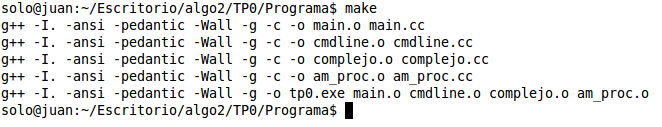
\includegraphics[width=1\textwidth]{compilacion.png}
	\caption{Compilación del programa.}
	\label{fig:corrida_makefile}
\end{figure}

En primera instancia se ve en la Figura \ref{fig:corrida_makefile} que la compilación del programa resulta satisfactoria según lo desarrollado en la sección \ref{sec:comp}.

Luego se probaron los ejemplos propuestos por las especificaciones:

\begin{figure}[H]
	\centering
		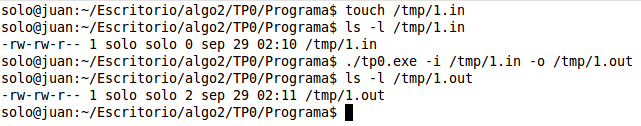
\includegraphics[width=1\textwidth]{prueba-1_con_problemas.png}
	\caption{Ejemplo 1 del enunciado del TP.}
	\label{fig:prueba1_con_prob}
\end{figure}


\begin{figure}[H]
	\centering
		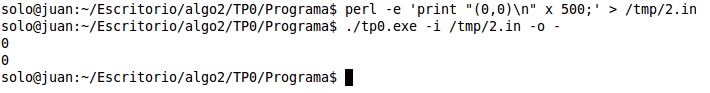
\includegraphics[width=1\textwidth]{prueba-2_con_problemas.png}
	\caption{Ejemplo 2 del enunciado del TP.}
	\label{fig:prueba2_con_prob}
\end{figure}

\begin{figure}[H]
	\centering
		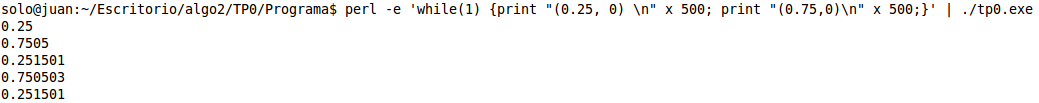
\includegraphics[width=1\textwidth]{prueba-3_con_problemas.png}
	\caption{Ejemplo 3 del enunciado del TP.}
	\label{fig:prueba3_con_prob}
\end{figure}

Como se puede ver en las Figuras \ref{fig:prueba1_con_prob} y \ref{fig:prueba2_con_prob}, el programa imprime un número por demás. Esto evidencia que al encontrarse con el final del archivo, vuelve a imprimir un complejo (algo que no debería suceder). Analizando el código se encontró el origen del error en el archivo \texttt{am\_proc.cc}

\begin{lstlisting}[firstnumber=100]
	if (is->eof())
		eof_flag=true;
\end{lstlisting}

A partir de este código se ve que al encontrar EOF cambia el valor de \texttt{eof\_flag} y continua con los demás comandos dentro del bucle, entre ellos la decimación e impresión. Si se insertan exactamente \texttt{N} complejos, ocurre una iteración indeseada. Para solucionar dicho problema se implementó lo siguiente

\begin{lstlisting}
	if(is->eof()){
		eof_flag=true;
		if(c==0)
			break;
	}
\end{lstlisting}

Se corrieron nuevamente las pruebas anteriores y a continuación se presentan los resultados

\begin{figure}[H]
	\centering
		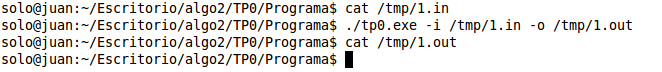
\includegraphics[width=1\textwidth]{prueba-1.png}
	\caption{Ejemplo 1 del enunciado del TP funcionando correctamente.}
	\label{fig:prueba1}
\end{figure}

\begin{figure}[H]
	\centering
		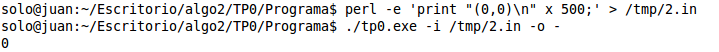
\includegraphics[width=1\textwidth]{prueba-2.png}
	\caption{Ejemplo 2 del enunciado del TP funcionando correctamente.}
	\label{fig:prueba2}
\end{figure}

Además, para probar si se obtiene el resultado correcto al insertar una cantidad que no sea múltiplo del número de decimación, se ejecutó el siguiente \emph{test}

\begin{figure}[H]
	\centering
		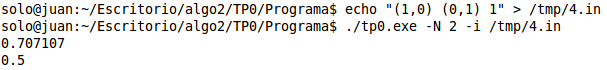
\includegraphics[width=1\textwidth]{prueba-5.png}
	\caption{Prueba al insertar una cantidad indivisible por el número de decimación}
	\label{fig_prueba5}
\end{figure}

Al mismo tiempo, se analizó el problema presentado en la Figura \ref{fig:prueba3_con_prob}. La causa de que los resultados tuvieran errores en los últimos 4 decimales fue la falta de inicialización de \texttt{c} al comenzar nuevamente el ciclo \texttt{while} del archivo \texttt{am\_proc.cc}. Ésto se solucionó de la siguiente manera:

\begin{lstlisting}
	for(i=1, c=0; i<=n_decimator && ((*is)>>aux); i++)
\end{lstlisting}

\begin{figure}[H]
	\centering
		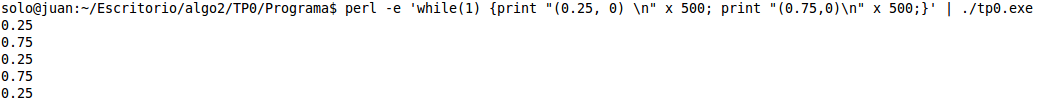
\includegraphics[width=1\textwidth]{prueba-3.png}
	\caption{Ejemplo 3 del enunciado del TP.}
	\label{fig:prueba3}
\end{figure}

Como se puede ver en la Figura \ref{fig:prueba3}, la implementación propuesta logró solucionar el problema previo. Cabe destacar que las capturas de pantalla expuestas, se realizaron al resolver ambos problemas en simultaneo. De lo contrario, la prueba de la Figura \ref{fig_prueba5} hubiera tenido el mismo error presentado por el problema original.

Por otro lado, se puso a prueba la interpretación de los números complejos. Se prueba si al ingresar una serie de coeficientes como la parte real, origina el mismo resultado que los mismos coeficientes pero como parte puramente imaginaria. En la siguiente Figura se exponen las corridas:

\begin{figure}[H]
	\centering
		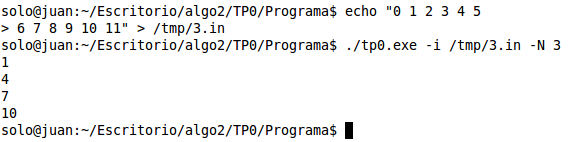
\includegraphics[width=1\textwidth]{prueba-4.png}
\end{figure}
\begin{figure}[H]
	\centering
		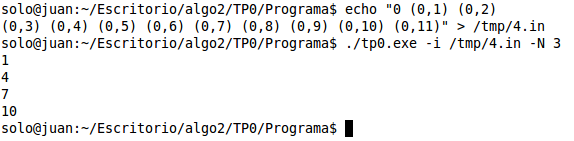
\includegraphics[width=1\textwidth]{prueba-4bis.png}
	\caption{Prueba con distintos números complejos}
	\label{fig:prueba-4}
\end{figure}

Finalmente se insertó una cadena de caracteres para ver cómo se comporta el programa ante un error en la entrada y el resultado, satisfactorio, se puede ver a continuación:

\begin{figure}[H]
	\centering
		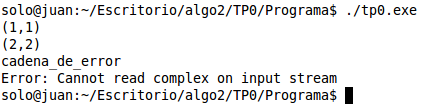
\includegraphics[width=1\textwidth]{prueba-6.png}
	\caption{Prueba ingresando no-complejos}
	\label{fig:prueba-6}
\end{figure}

